\documentclass[xcolor=dvipsnames, notes]{beamer}
%\documentclass[xcolor=dvipsnames]{beamer}

\usetheme{Warsaw}

\usepackage{amsmath}
\usepackage{amsthm}
\usepackage{graphicx}

\title{Sequential Reasoning for Optimizing Compilers Under Weak Memory Concurrency}
\subtitle{Minki Cho, Sung Hwan Lee, Dongjae Lee, Chung Kil Hur, Ori Lahav}

\author{Presented by \\ Akshay Gopalakrishnan}

\begin{document}

    \begin{frame}
        
        \maketitle

    \end{frame}


    \begin{frame}{Introduction}
        
        \begin{itemize}
            \item Performing/designing thread-local optimizations in a concurrent context would require understanding the underlying memory consistency model.
            \item Often, these models are complex, as they are weak consistency based.
            \item Thus, it becomes difficult to design optimizations which are safe.
            \item Most optimizations that are performed on concurrent programs mainly involve reordering or eliminating non-atomics.
            \item Is there perhaps, then a simpler semantics that an optimization designer can rely on?
        \end{itemize}

    \end{frame}

    %Should take about 1hr to do and finish off
    \begin{frame}{Main Idea}
        
        \begin{itemize}
            \item This paper proposes a Sequential Model (SEQ) to design compiler optimizations.
            \item The optimizations addressed are solely regarding non-atomics, or reordering non-atomics across atomic parts of code. 
            \item SEQ is shown to preserve contextual refinement for non-atomic optimizations in the Promising Semantics (PS).
            \item Contextual refinement in PS makes sure that optimization developers can solely on SEQ to design optimizations.  
        \end{itemize}

    \end{frame}

    \begin{frame}{Optimizations on Non-atomics}

        \begin{itemize}
            \item Reordering non-atomics (RR/WR/WW/RW).
            \item Reordering non-atomics outside loops (Loop Invariant Code motion).
            \item Elimination of non-atomics (RR/WR/WW/RW).
            \item Redundant non-atomic load introduction/elimination. 
            \item Reordering atomics with non-atomics (RR/WR/WW/RW).
            \item Elimination of non-atomics across atomics.  
        \end{itemize}
        
    \end{frame}

    \note{
        The non-adjacent optimization involving elimination of non-atomics across atomics does not seem to be required in my opinion.
        This is because the proof for that can be justified by decomposing the optimizations into the above elementary adjacent components.

        To add, Write introduction is not allowed by the model. 
        This is a good design choice to preserve security guarantees, however it still limits from introducing redundant writes within dead-code blocks, which may be used by optimizing compilers to easily perform partial redundancy elimination.
    }
    
    \begin{frame}{SEQ Machine: Memory Events and State}

        \begin{itemize}
            \item Atomic events of Type RLX/REL/ACQ.
            \item Non atomic events of type NA.
        \end{itemize}

        Each state $S = \langle \alpha , P, F , M \rangle$ keeps track of
        \begin{itemize}
            \item $\alpha$ - State transition.
            \item $P$ - Permission set, has set of non-atomic locations safe to access.
            \item $F$ - Written set, has set of non-atomic locations written to. 
            \item $M$ - Shared memory set, consisting both atomic and non-atomic locations. 
        \end{itemize}
    
        Final state is either $return \ v$ or $\bot$ (which includes undefined behavior).
        
    \end{frame}

    \note{
        It is unclear whether $P$ at the beginning of the execution includes all possible non-atomic locations (is it $\top$) or it is empty (is it $\bot$).
        My understanding is that it should be $\bot$, and that acquire semantics would start including in the set locations we are safe to read/write to, whereas release semantics would do the reverse.
        The transitions seem to make sense, the non-deterministic change (inclusion in acq and exclusion in rel) is meant to reflect any random context (other threads) that would be running concurrently.
    }

    \begin{frame}{SEQ Machine 1: State Transitions}

        %Add figure here of the state transitions.
        \begin{figure}
            \makebox[\textwidth][c]{
                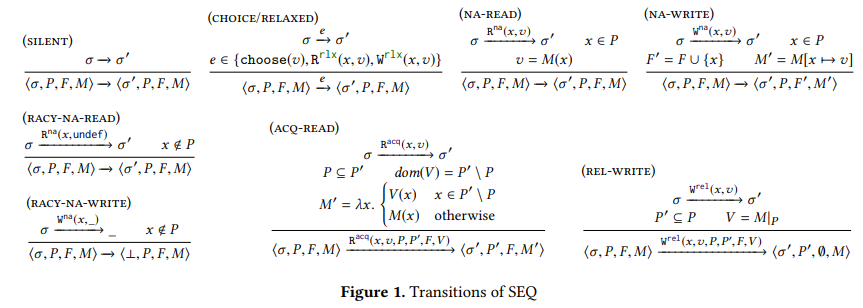
\includegraphics[scale=0.7]{SEQ_Simple.png}
            }
        \end{figure}

        
    \end{frame}


    \begin{frame}{Towards Soundness of Optimizations}

        A Behavior is defined as $\langle tr, r \rangle$ where
        \begin{itemize}
            \item $tr$ is the sequence of labels denoting an in which a trace of events were executed.
            \item $r$ is either 
            \begin{itemize}
                \item $trm(v, F, M)$ denoting return value $v$, updated writes $F$ and memory state $M$.
                \item $\bot$ denoting erroneous termination, which includes Undefined behavior.
            \end{itemize}  
        \end{itemize}
        
    \end{frame}

    \begin{frame}{Refinement of Transition Steps}

        %Put figure here of the transition steps
        \begin{figure}
            \makebox[\textwidth][c]{
                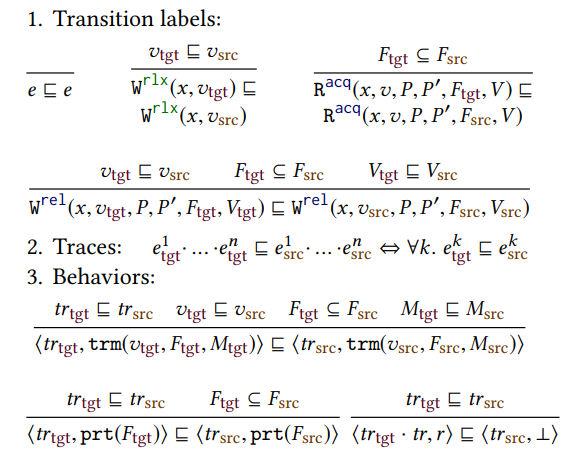
\includegraphics[scale=0.7]{SEQ_Refinement.png}
            }
        \end{figure}

        
    \end{frame}

    \note{
        What baffles me is the last transition, which says the normal termination is a refinement of erroenous termination. 
        I guess this means it is okay to make something that invokes undefined behavior to one that does not. 
        In the context of data races however, this would clearly be incorrect, since removing races, even if desirable is not the original behavior of the program.
        The compiler is allowed to do anything yes, but I guess from a debugging standpoint this would not be ideal.
        Perhaps mail one of the authors about this.
    }

    \begin{frame}{Problem with Simple SEQ}

        \begin{itemize}
            \item Reordering of non-atomics across atomics in certain cases are unsound.
            \item Most of these cases reduce to \textit{Roach Motel Reordering}.
            \item Reason is the final set of labels are different, keeping the termination state as $\bot$.
            \item Example: $a = y^{rlx}; b = x ^{na} \mapsto b = x^{na}; a = y^{rlx}$.
        \end{itemize}
        
    \end{frame}

    \begin{frame}{Fixes: High Level}

        \begin{itemize}
            \item Relax the definition of $\sqsubseteq$ on trace labels.
            \item Handle rlx-na to na-rlx: Assume no fixed read value returned for an atomic read. 
            \item Handle acq-na to na-acq: Restrict $tr$ of source such that the sequence of labels contain no acquire reads that lead to UB.
            \item Handle rel-na to na-rel: Commitment set of non-atomic writes to be fulfilled before an acquire read.
        \end{itemize}
        
    \end{frame}

    \note{
        The solution to address the disallowing of non-atomic and atomic reordering is certainly confusing. 
        While some of it is intuitive, it does not give the confidence that it actually would hold in all cases.
        The crux is to relax the refinement definition to incorporate more reorderings, noting that some information of trace labels are irrelevant.
        \begin{itemize}
            \item The first idea is to note that if you anyways reach UB irrespective of reordering, then you can make do by not ensuring all trace labels are the same.
            \item To ensure we do not mess this up, we need to ensure that we do not introduce UB by reordering across acquire reads (as hb relation would make sure no data race in some sense). This translates to ensuring the trace labels have no trailing acquire reads.
            \item Next, to ensure we do not introduce UB again by optimizing, we should not assume the atomic reads have a fixed read value, assuming no fixed value of shared memory. 
            \item Lastly, to ensure we can reorder non-atomics writes before release writes, we need to ensure the source program can commit the writes after the release (this one is confusing).  
        \end{itemize}
    }

    \begin{frame}{Towards Adequacy of SEQ}

        The main claim for SEQ was that a compiler developer can solely rely on sequential semantics (SEQ in this case) to design sound optimizations (that which satisfy contextual refinement). 
        \begin{itemize}
            \item Adequacy of SEQ is shown by claiming any optimization (refinement) sound in SEQ is sound in Promising Semantics.
            \item Adequacy is contingent on program being deterministic, that concrete execution path always leads to the same final outcome.
        \end{itemize}
        
    \end{frame}

    \begin{frame}{Assumptions/Limitations}

        \begin{itemize}
            \item Do not tackle optimizations only involving atomics, claiming this is rarely done by compilers. 
            \item LICM tackled only involves removing read-events outside the loop, what about writes? Usually writes are not involved or considered as a Loop invariant. 
            \item SEQ thus, cannot be used for atomic optimizations, and thus atomic based optimizations would require understanding PS at its full.
            \item SEQ relies on the practical implementation and usage of Promising Semantics as a programming language model.
            \item Paper claims it addresses optimizations without catch-fire semantics, but still uses a notion of UB from LLVM semantics to prove soundness of optimizations. 
            \item Paper's claims on optimizations are additive, with minor warnings on allowing false optimizations. However, it is not yet clear if it allows only what is desired.
        \end{itemize}
        
    \end{frame}

    \begin{frame}{Conclusion}

        \begin{itemize}
            \item Paper seemed to falsify the rhetoric. The intention being to allow non-atomic based optimizations in the PS. 
            \item This was done by designing a simpler sequential model SEQ, taking advantage of UB and being conservative while proving contextual refinement. 
            \item SEQ was then showed \text{COMPLETE} w.r.t. PS for the intended optimizations.
            \item Promising Semantics was extended by adding non-atomic events (did not discuss here in this presentation).
        \end{itemize}
        
    \end{frame}

\end{document}